% Póster del TPF: 70 x 100 cm, una página.
% Las figuras salen de poster/figuras_poster.py. Compilar dos veces con lualatex.
\documentclass{article}
\usepackage[paperwidth=700mm, paperheight=1000mm, margin=0mm]{geometry}
\usepackage{fontspec}
\usepackage{unicode-math}
\setmainfont{FiraSans}[
  Extension = .otf,
  UprightFont = *-Regular,
  BoldFont = *-SemiBold,
  ItalicFont = *-Italic,
  BoldItalicFont = *-SemiBoldItalic,
]
\setmathfont{FiraMath-Regular.otf}
\usepackage{xcolor}
\usepackage{graphicx}
\usepackage{qrcode}
\usepackage{tikz}
\usetikzlibrary{arrows.meta, calc, positioning}

\definecolor{tinta}{HTML}{1D2433}
\definecolor{tinta2}{HTML}{4A5160}
\definecolor{suave}{HTML}{8A90A0}
\definecolor{linea}{HTML}{DCDCD6}
\definecolor{entrada}{HTML}{B5604E}
\definecolor{metodo}{HTML}{2A78D6}
\definecolor{suavizado}{HTML}{EB6834}
\definecolor{simetria}{HTML}{1BAF7A}
\definecolor{original}{HTML}{7E848A}
\definecolor{paper}{HTML}{EEF0F3}

\pagestyle{empty}
\setlength{\parindent}{0pt}
\setlength{\parskip}{0pt}
\hyphenpenalty=10000
\exhyphenpenalty=10000
\color{tinta}

\newcommand{\cuerpo}{\fontsize{27}{35}\selectfont}
\newcommand{\chico}{\fontsize{22}{28}\selectfont}
\newcommand{\diminuto}{\fontsize{18}{23}\selectfont}

% Encabezado de sección: número en un círculo y título.
\newcommand{\seccion}[2]{%
  {\fontsize{44}{50}\selectfont
   \tikz[baseline=(n.base)]\node[circle, fill=tinta, text=white, inner sep=0pt,
     minimum size=16mm, font=\fontsize{32}{32}\selectfont\bfseries](n){#1};%
   \hspace{5mm}\textbf{#2}\par}%
  \vspace{6mm}}

\newcommand{\punto}[1]{%
  \hangindent=7mm\hangafter=1
  \makebox[7mm][l]{\textcolor{suave}{\textbullet}}#1\par\vspace{2.5mm}}

% Entrada de la lista de referencias, con sangría francesa.
\newcommand{\bib}[1]{\par\vspace{0.6mm}\hangindent=9mm\hangafter=1\makebox[9mm][l]{[#1]}}

% Rótulo de una columna de figura, centrado en un ancho dado.
\newcommand{\rotulo}[3]{\makebox[#1][c]{\textcolor{#2}{\bfseries #3}}}

% TikZ fija \spaceskip en em del tamaño de letra del nodo: se vuelve al espacio de cada fuente.
\newcommand{\espacios}{\spaceskip=0pt\xspaceskip=0pt\relax}

% Ubicación absoluta: \bloque{x}{y}{ancho}{contenido}, en mm desde la esquina superior
% izquierda. Sin la opción align de TikZ, que fija el espacio entre palabras al tamaño de
% letra del nodo.
\newcommand{\bloque}[4]{%
  \node[anchor=north west, inner sep=0pt, text width=#3mm]
    at ($(current page.north west) + (#1mm, -#2mm)$) {\espacios\raggedright #4};}

\tikzset{
  every node/.append style={execute at begin node=\espacios},
  etapa/.style={draw=suave, fill=paper, rounded corners=3mm, line width=1.2mm,
    minimum height=23mm, text width=47mm, align=center, inner sep=2mm,
    font=\fontsize{22}{26}\selectfont},
  propia/.style={etapa, line width=1.8mm, font=\fontsize{22}{26}\selectfont\bfseries},
  flecha/.style={-{Latex[length=6mm, width=6mm]}, line width=1.3mm, draw=tinta2},
  rotulo/.style={font=\fontsize{19}{23}\selectfont, text=tinta2},
}

\begin{document}
\begin{tikzpicture}[remember picture, overlay]

% ---------------------------------------------------------------- encabezado
\fill[tinta] (current page.north west) rectangle ($(current page.north east) + (0, -104mm)$);
\bloque{25}{11}{490}{%
  {\fontsize{112}{116}\selectfont\bfseries\color{white} Completar mallas rotas\par}
  \vspace{7mm}
  {\fontsize{34}{43}\selectfont\color{white!78!tinta}
   Una extensión de Jacobson, Kavan y Sorkine-Hornung (SIGGRAPH 2013) con suavizado
   de tapas y completación por simetría\par}}
\node[anchor=north east, inner sep=0pt, text width=150mm]
  at ($(current page.north east) + (-25mm, -19mm)$) {\espacios\raggedleft\color{white}
  {\fontsize{40}{50}\selectfont\bfseries Lucas Allara\par}
  \vspace{5mm}
  {\fontsize{30}{40}\selectfont\color{white!78!tinta}
   Computación Gráfica\\ Universidad Torcuato Di Tella\\ 2.º cuatrimestre de 2026\par}};

% ---------------------------------------------------------------- teaser
\bloque{25}{116}{650}{%
  \fontsize{30}{36}\selectfont
  \rotulo{130mm}{entrada}{Entrada}%
  \rotulo{130mm}{metodo}{Método de [1]}%
  \rotulo{130mm}{suavizado}{Con suavizado}%
  \rotulo{130mm}{simetria}{Con suavizado y simetría}%
  \rotulo{130mm}{original}{Original}\par
  \vspace{3mm}
  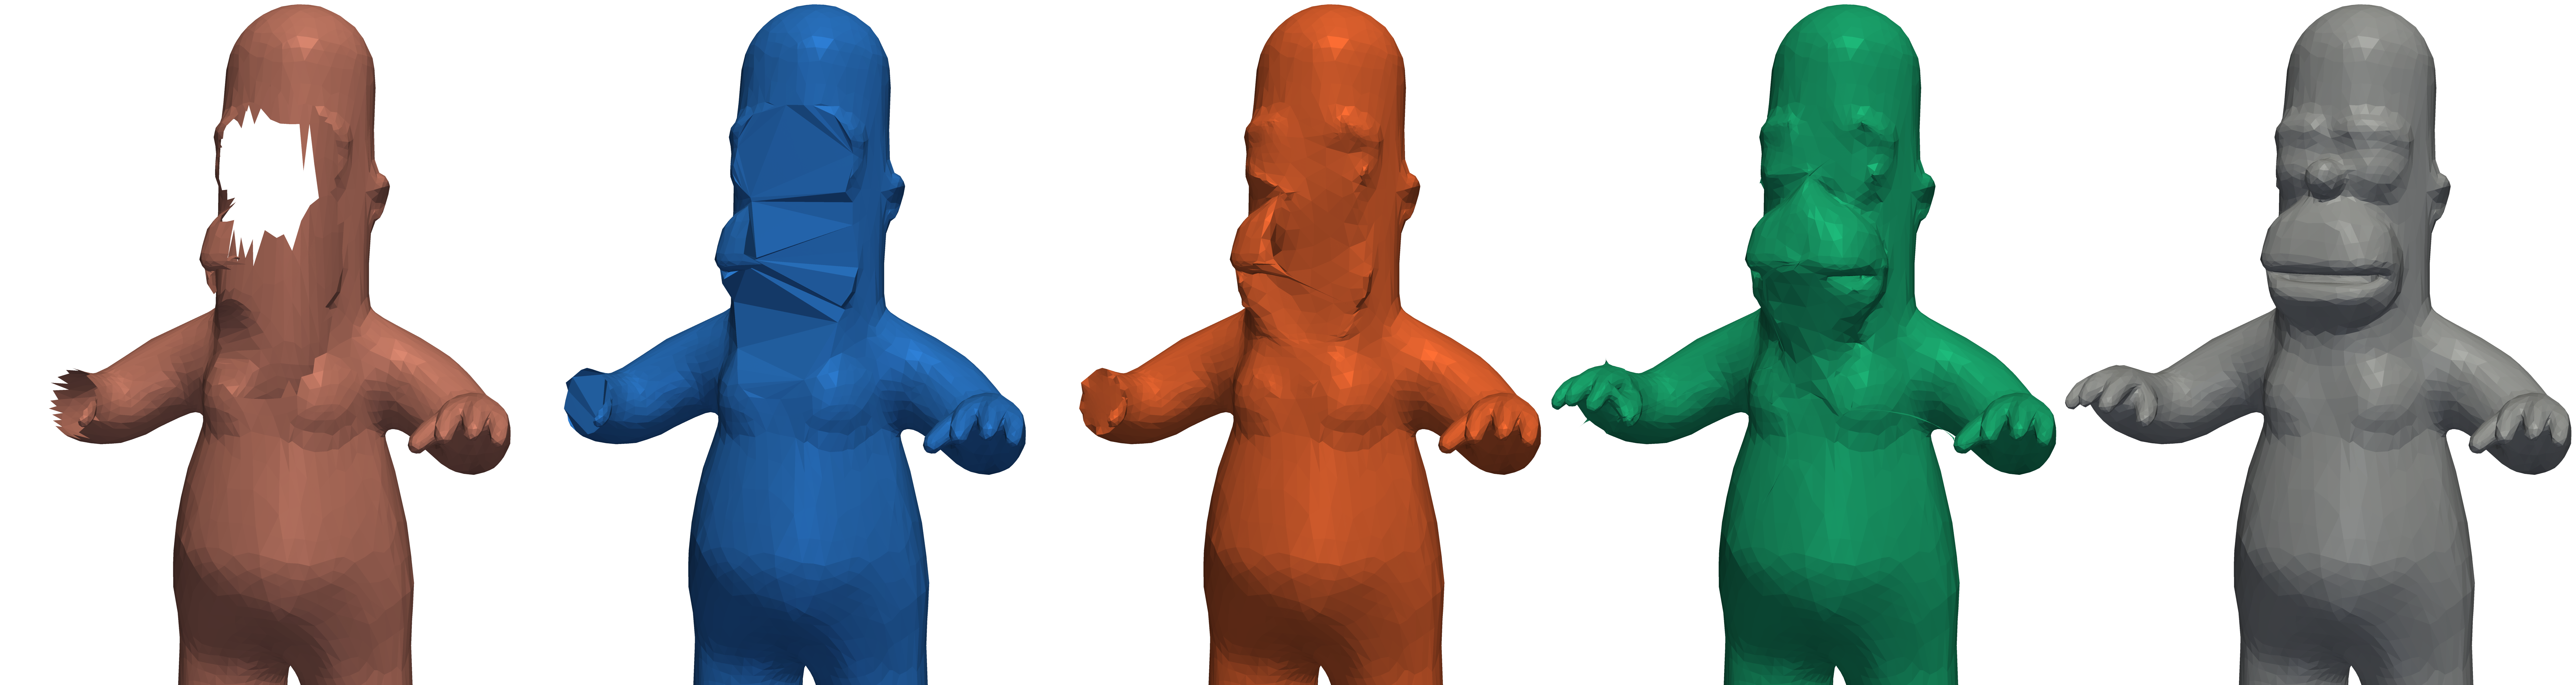
\includegraphics[width=650mm, trim=0 300 0 0, clip]{figuras/teaser.png}\par}

% ---------------------------------------------------------------- 1
\bloque{25}{293}{305}{%
  \seccion{1}{Introducción}
  {\cuerpo Muchas mallas reales tienen agujeros, piezas superpuestas o caras sueltas, y para
   simular o imprimir un modelo hace falta saber qué puntos están dentro. Jacobson et al.\ [1]
   usan el número de vueltas generalizado, que suma los ángulos sólidos con que se ven las
   caras desde \(p\).\par}
  \vspace{3mm}
  {\centering\fontsize{38}{46}\selectfont
   \(w(p) = \dfrac{1}{4\pi} \displaystyle\sum_{f} \Omega_f(p)\)\par}
  \vspace{2mm}
  {\centering
   \begin{minipage}{150mm}
     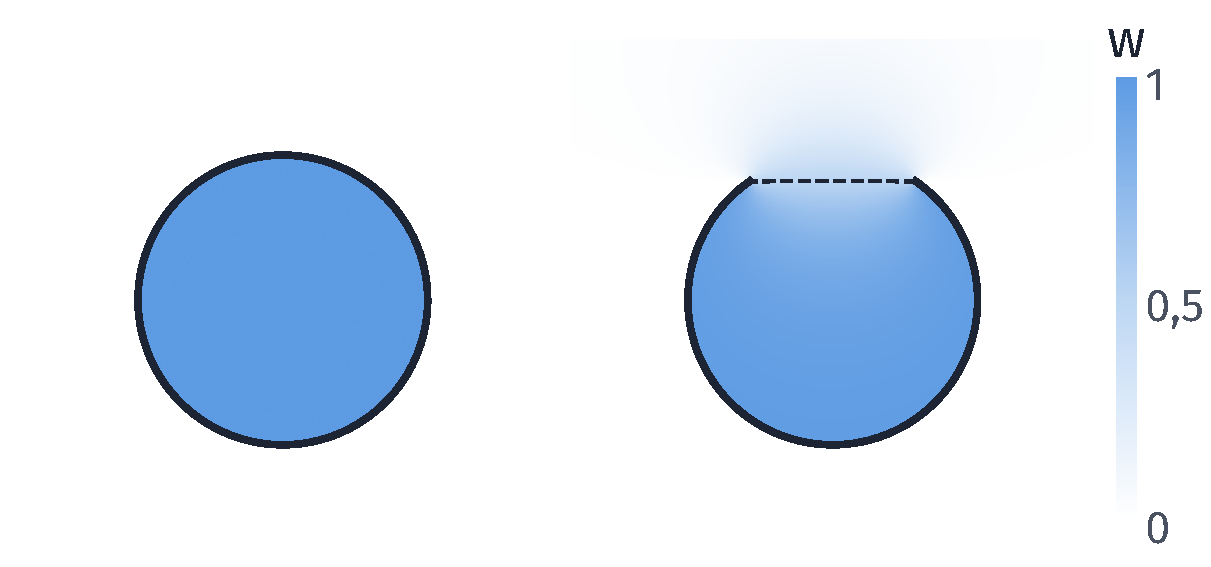
\includegraphics[width=150mm]{figuras/corte_w.pdf}\par
     {\chico\color{tinta2}
      \rotulo{68mm}{tinta2}{malla cerrada}\rotulo{68mm}{tinta2}{con un agujero}\par}
   \end{minipage}\par}
  \vspace{4mm}
  {\cuerpo Se tetraedriza el espacio respetando las caras de entrada [2], se evalúa \(w\) en
   cada tetraedro y un corte de grafo elige cuáles quedan adentro, penalizando separar vecinos
   parecidos. Dos heurísticas corrigen el resultado para que la salida, el borde de esa región,
   contenga las caras de entrada y sea una variedad.\par}}

% ---------------------------------------------------------------- 2
\bloque{360}{293}{315}{%
  \seccion{2}{Propuesta}
  {\cuerpo Donde faltaba superficie, la salida de [1] está hecha de caras de la
   tetraedrización, que cierran el agujero con triángulos planos y sin detalle. Se agregan dos
   etapas sin modificar las del método, tomando ideas del suavizado de TetWild [3] y de la
   completación por simetría [5].\par}
  \vspace{7mm}
  {\centering
   \begin{tikzpicture}[node distance=12mm and 11mm]
     \node[etapa, text width=34mm] (e1) {Entrada};
     \node[etapa, text width=92mm, right=of e1] (p1) {Tetraedrización,\\\(w\) y corte de grafo};
     \node[propia, draw=suavizado, fill=suavizado!12, text width=56mm, below=20mm of p1.south east,
       anchor=north west, xshift=11mm] (s2) {Suavizado\\\(\Delta^3 x = 0\)};
     \node[etapa, text width=34mm, below=20mm of e1] (e2) {Entrada};
     \node[etapa, text width=92mm, right=of e2] (p2) {Tetraedrización,\\\(w\) y corte de grafo};
     \node[etapa, text width=34mm, right=36mm of s2, draw=tinta, fill=white, line width=1.8mm,
       font=\fontsize{22}{26}\selectfont\bfseries] (o2) {Salida};
     \node[etapa, text width=34mm, draw=tinta, fill=white, anchor=center] (o1)
       at (o2.center |- p1.center) {Salida};
     \node[propia, draw=simetria, fill=simetria!12, text width=54mm, anchor=north] (r)
       at ($(p2.south)!0.5!(s2.south) + (0, -14mm)$) {Completar\\por simetría};
     \node[rotulo, anchor=south west, inner sep=0pt] at ($(e1.north west) + (0, 3mm)$)
       {\bfseries Método de [1]};
     \node[rotulo, anchor=south west, inner sep=0pt] at ($(e2.north west) + (0, 3mm)$)
       {\bfseries Propuesta};
     \draw[flecha] (e1) -- (p1);
     \draw[flecha] (p1) -- (o1);
     \draw[flecha] (e2) -- (p2);
     \draw[flecha] (p2) -- (s2);
     \draw[flecha] (s2) -- node[rotulo, above=1mm] {2.ª pasada} (o2);
     \draw[flecha, draw=simetria] (s2.south) |- node[rotulo, pos=0.3, right=2mm, text=simetria]
       {1.ª pasada} (r.east);
     \draw[flecha, draw=simetria] (r.west) -| node[rotulo, pos=0.75, left=2mm, text=simetria,
       align=right] {2.ª pasada, con las\\caras reflejadas} (p2.south);
   \end{tikzpicture}\par}
  \vspace{9mm}
  \begin{minipage}[t]{150mm}\espacios\raggedright
    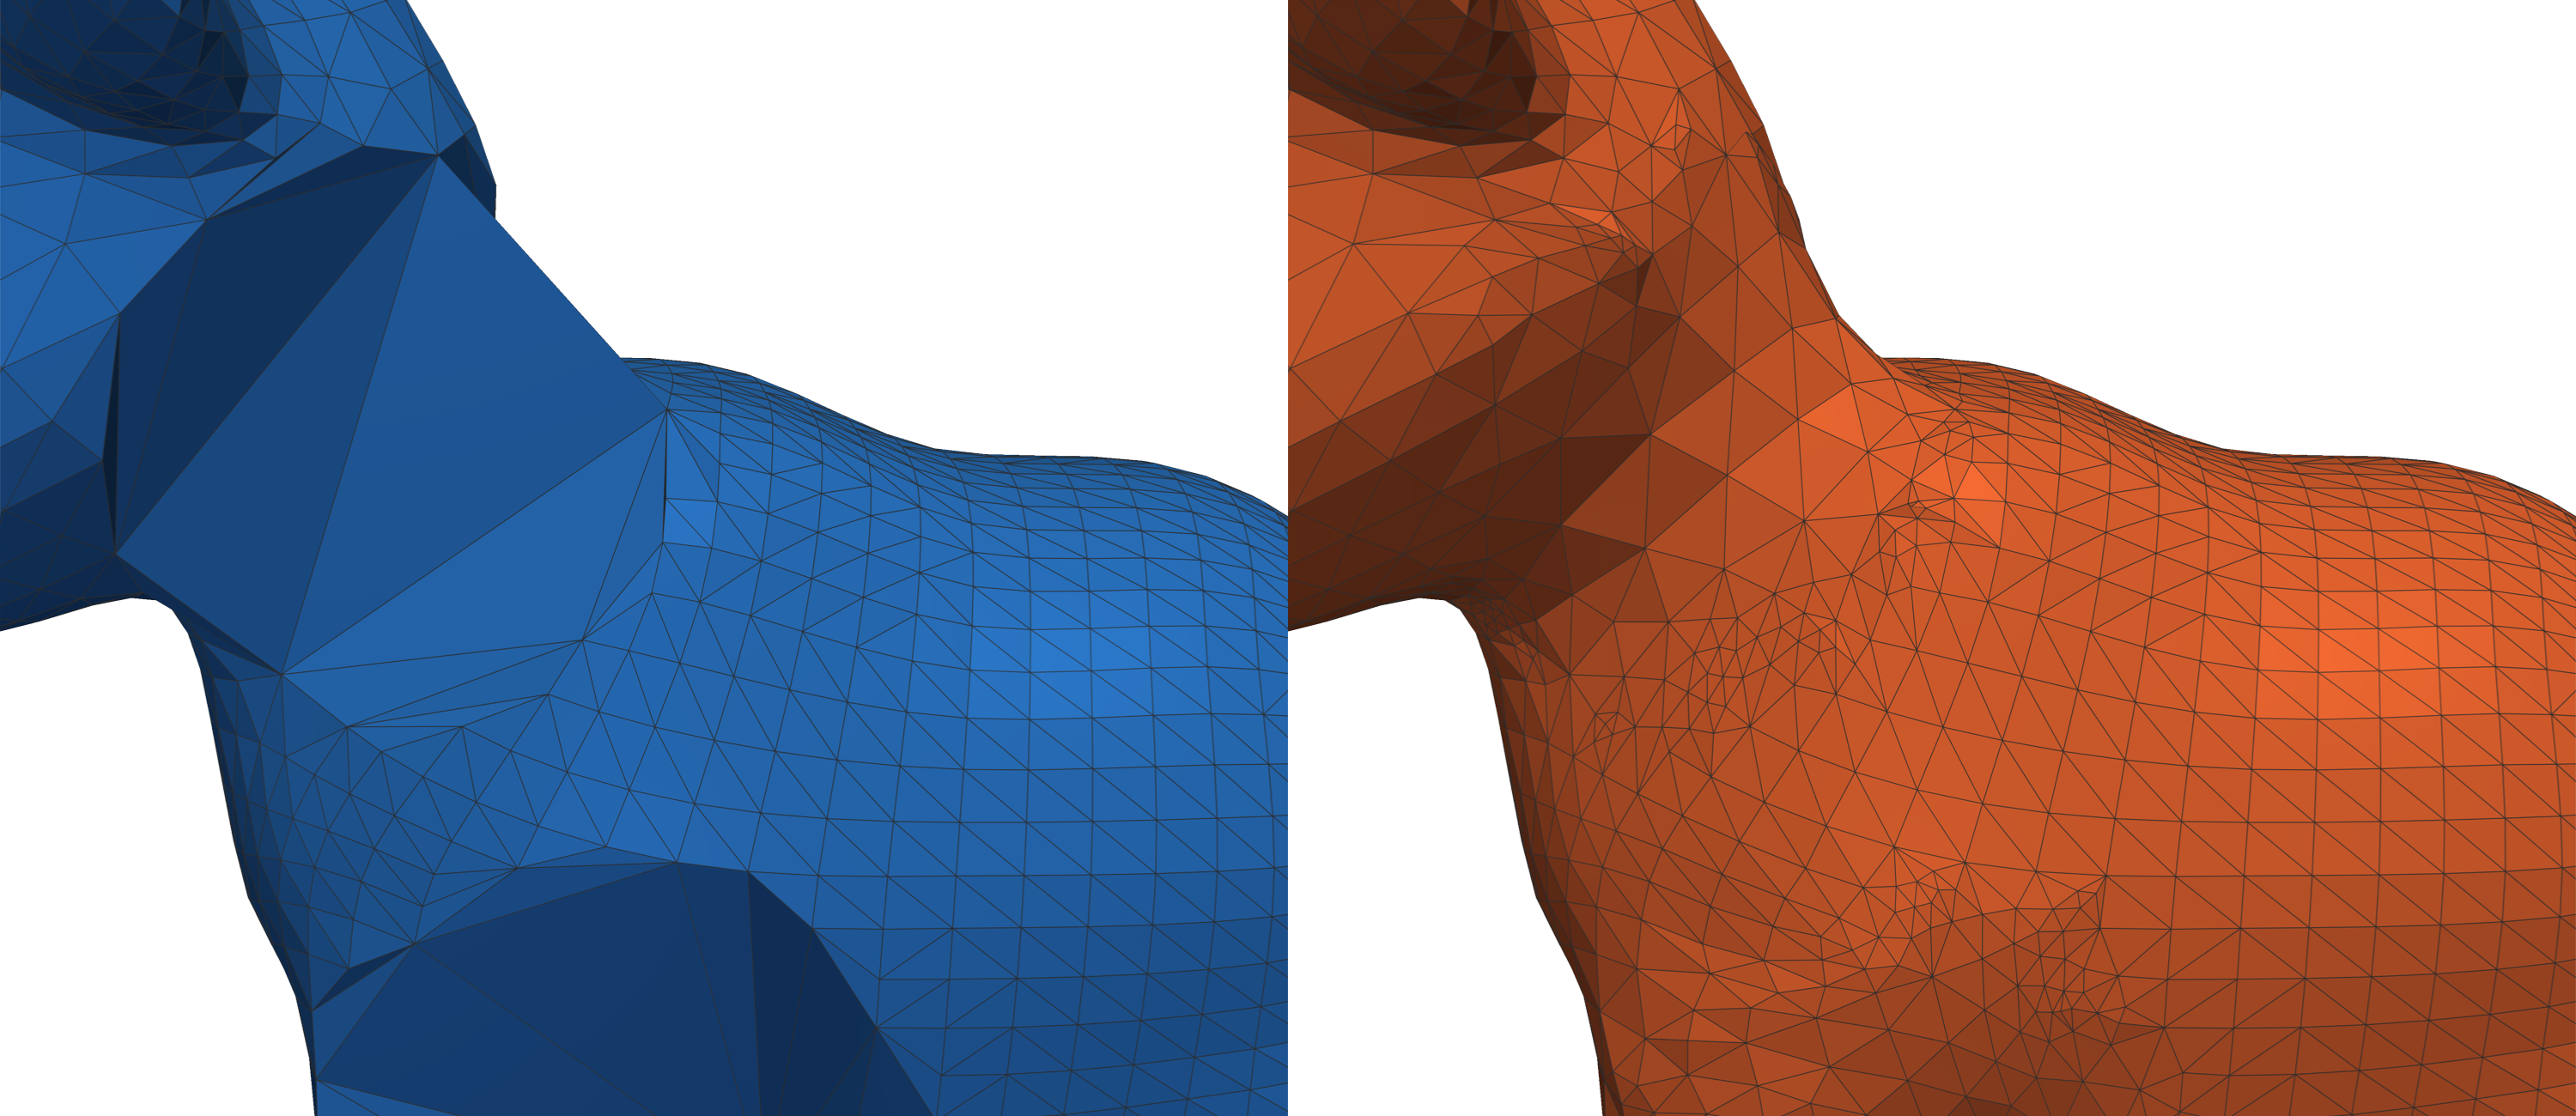
\includegraphics[height=60mm]{figuras/tapa.png}\par
    {\diminuto\rotulo{69mm}{metodo}{método de [1]}\rotulo{69mm}{suavizado}{con suavizado}\par}
    \vspace{3mm}
    {\chico\color{tinta2}
     \textcolor{suavizado}{\bfseries Suavizado.} La entrada queda fija y la tapa resuelve
     \(\Delta^3 x = 0\) [4], que la continúa en posición, tangente y curvatura.\par}
  \end{minipage}\hfill
  \begin{minipage}[t]{150mm}\espacios\raggedright
    \centering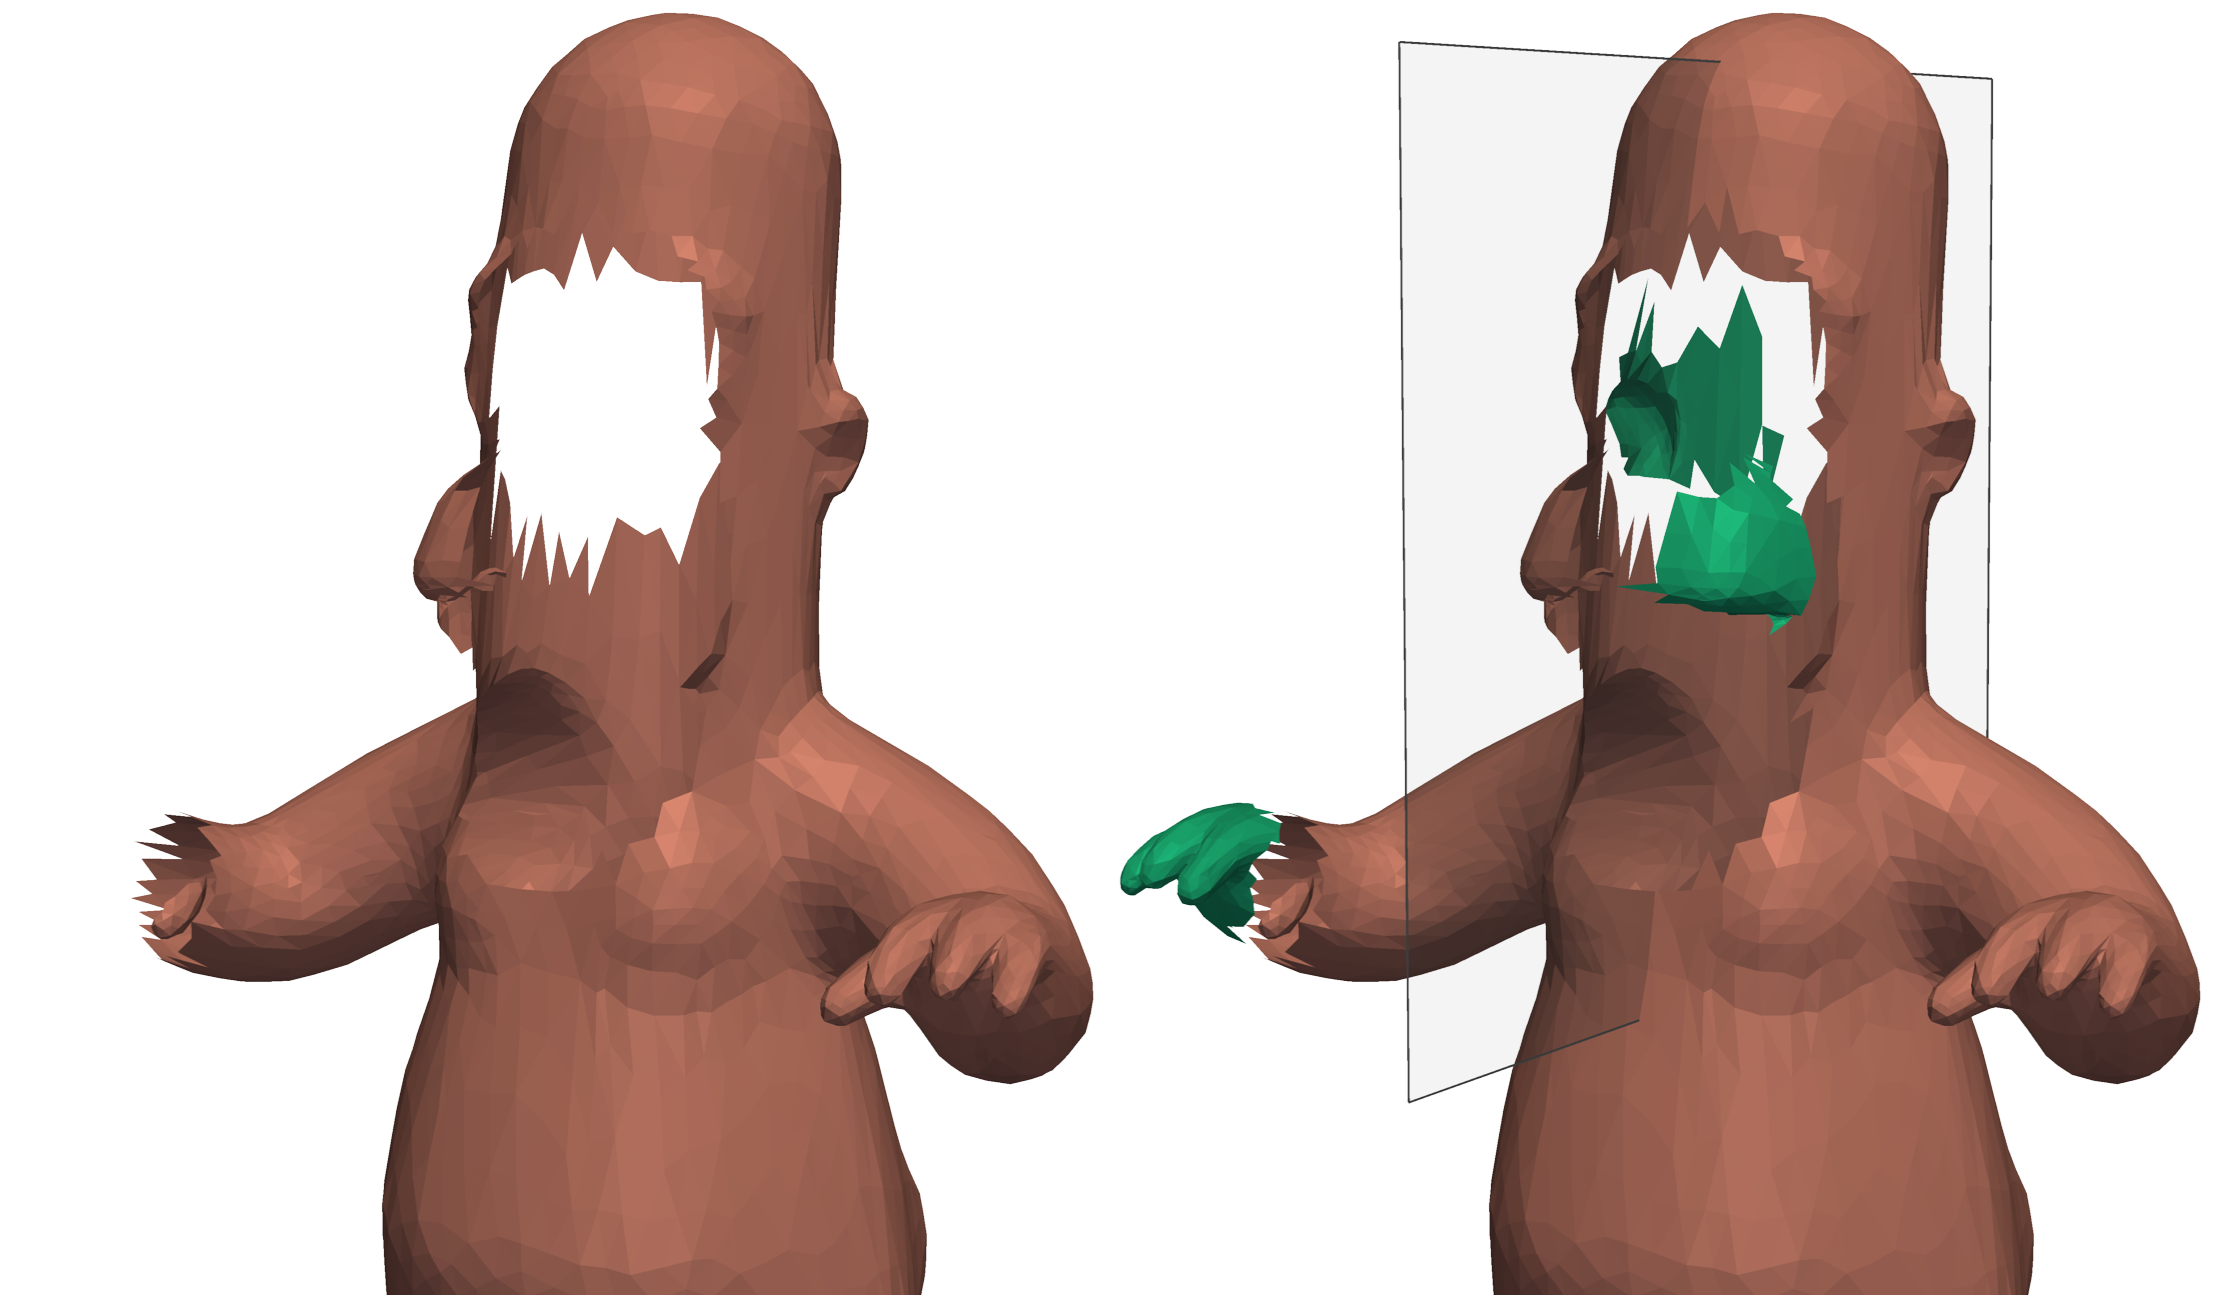
\includegraphics[height=60mm]{figuras/reflejo.png}\par
    {\diminuto\rotulo{51mm}{entrada}{entrada}\rotulo{51mm}{simetria}{caras reflejadas}\par}
    \vspace{3mm}\raggedright
    {\chico\color{tinta2}
     \textcolor{simetria}{\bfseries Simetría.} Se estima el plano de simetría y se agregan las
     caras reflejadas que caen en los agujeros.\par}
  \end{minipage}}

% ---------------------------------------------------------------- 3
\bloque{25}{581}{650}{\seccion{3}{Resultados}}
\bloque{25}{607}{350}{%
  \fontsize{22}{28}\selectfont
  \rotulo{70mm}{entrada}{Entrada}\rotulo{70mm}{metodo}{Método de [1]}%
  \rotulo{70mm}{suavizado}{Con suavizado}\rotulo{70mm}{simetria}{Con simetría}%
  \rotulo{70mm}{original}{Original}\par
  \vspace{3mm}
  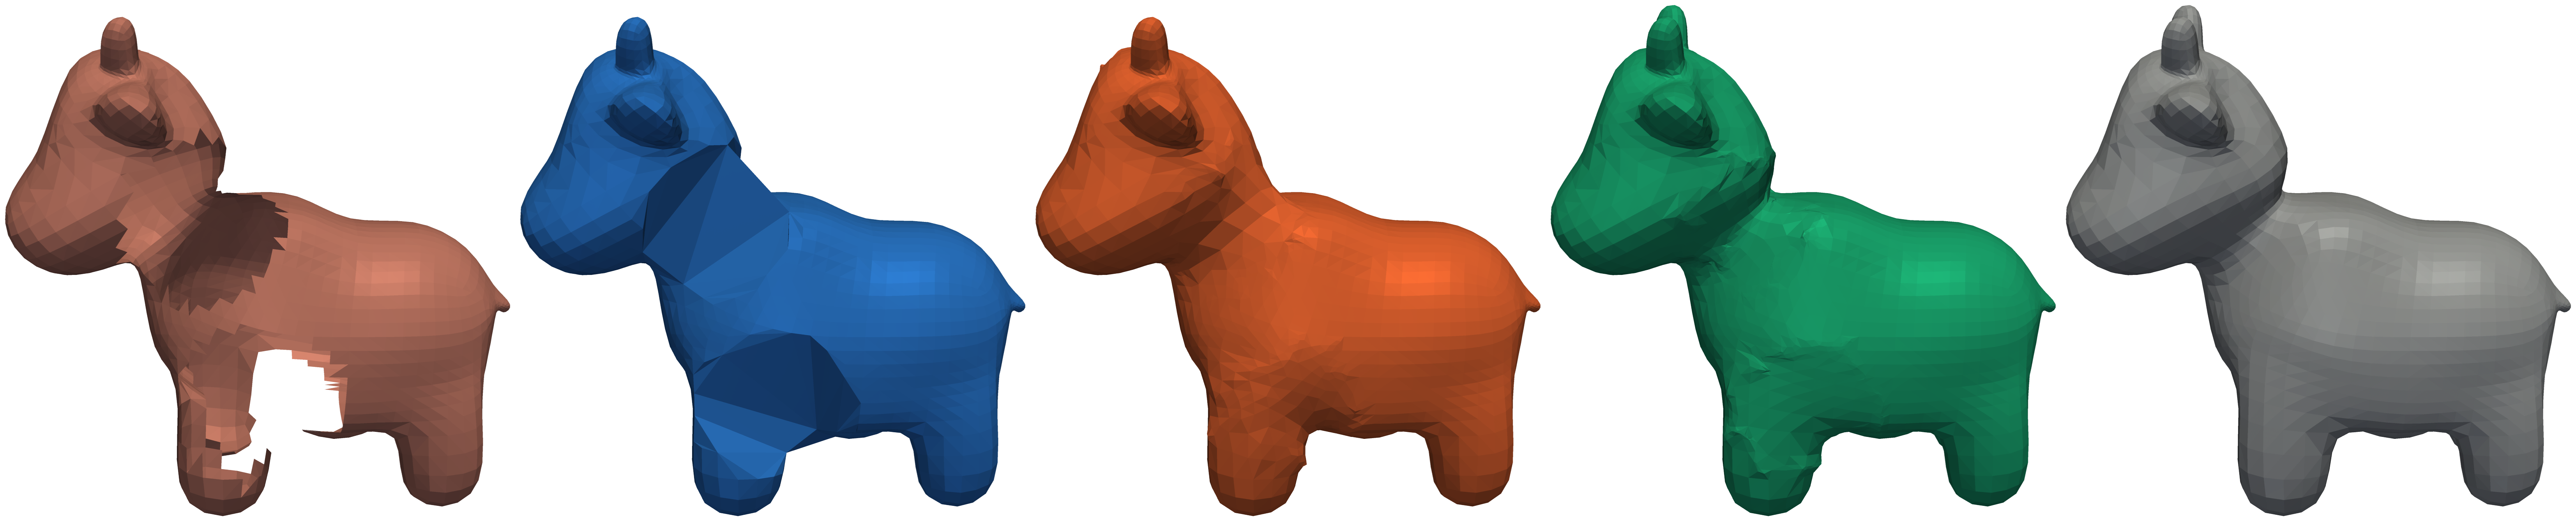
\includegraphics[width=350mm]{figuras/spot_22.png}\par
  \vspace{6mm}
  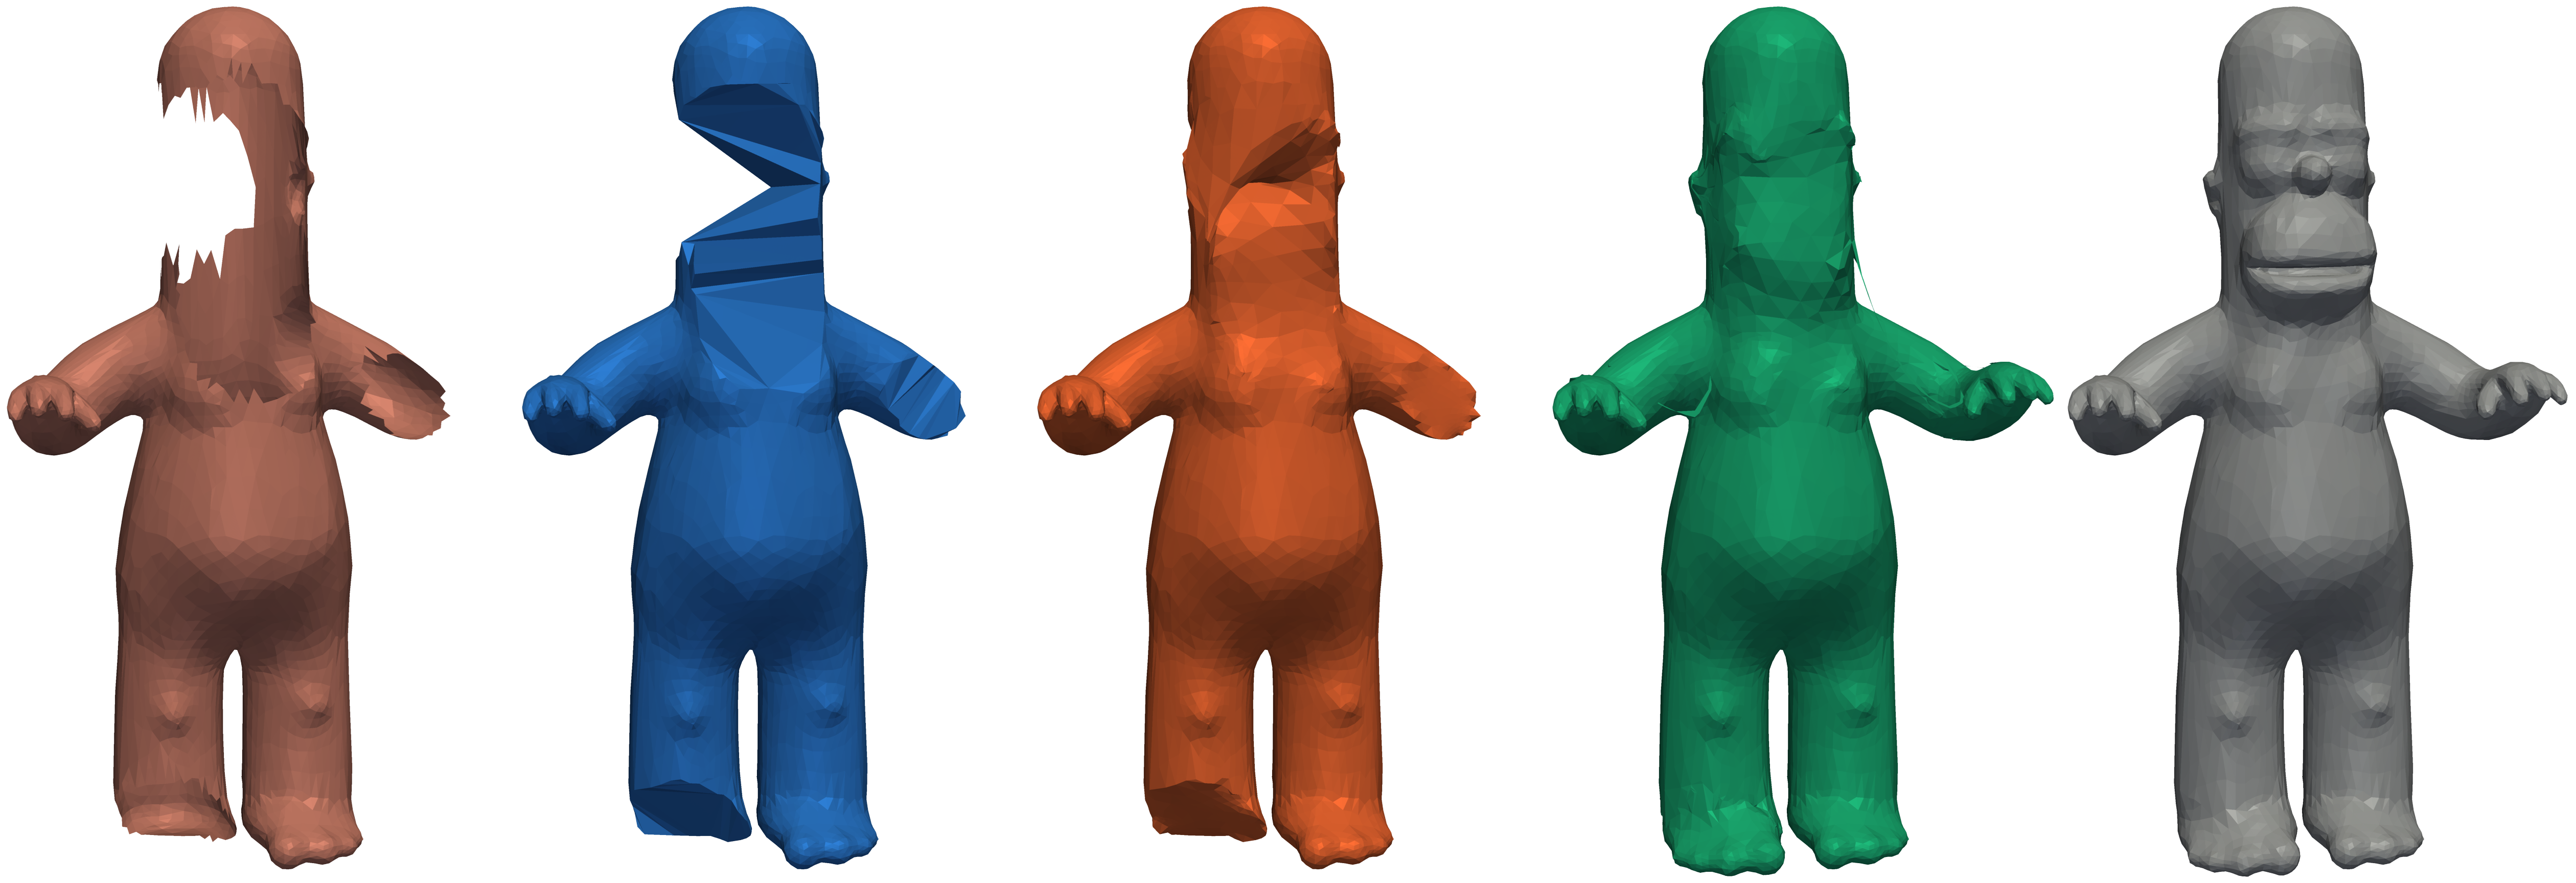
\includegraphics[width=350mm]{figuras/homer_22.png}\par}
\bloque{390}{611}{285}{%
  \begin{minipage}[t]{136mm}\espacios\raggedright
    {\fontsize{84}{88}\selectfont\bfseries\color{suavizado} −43\,\%\par}
    \vspace{2mm}
    {\chico error medio en los agujeros con el suavizado. Mejora los 18 casos.\par}
  \end{minipage}\hfill
  \begin{minipage}[t]{136mm}\espacios\raggedright
    {\fontsize{84}{88}\selectfont\bfseries\color{simetria} −79\,\%\par}
    \vspace{2mm}
    {\chico con suavizado y simetría. También mejora los 18 casos.\par}
  \end{minipage}\par
  \vspace{5mm}
  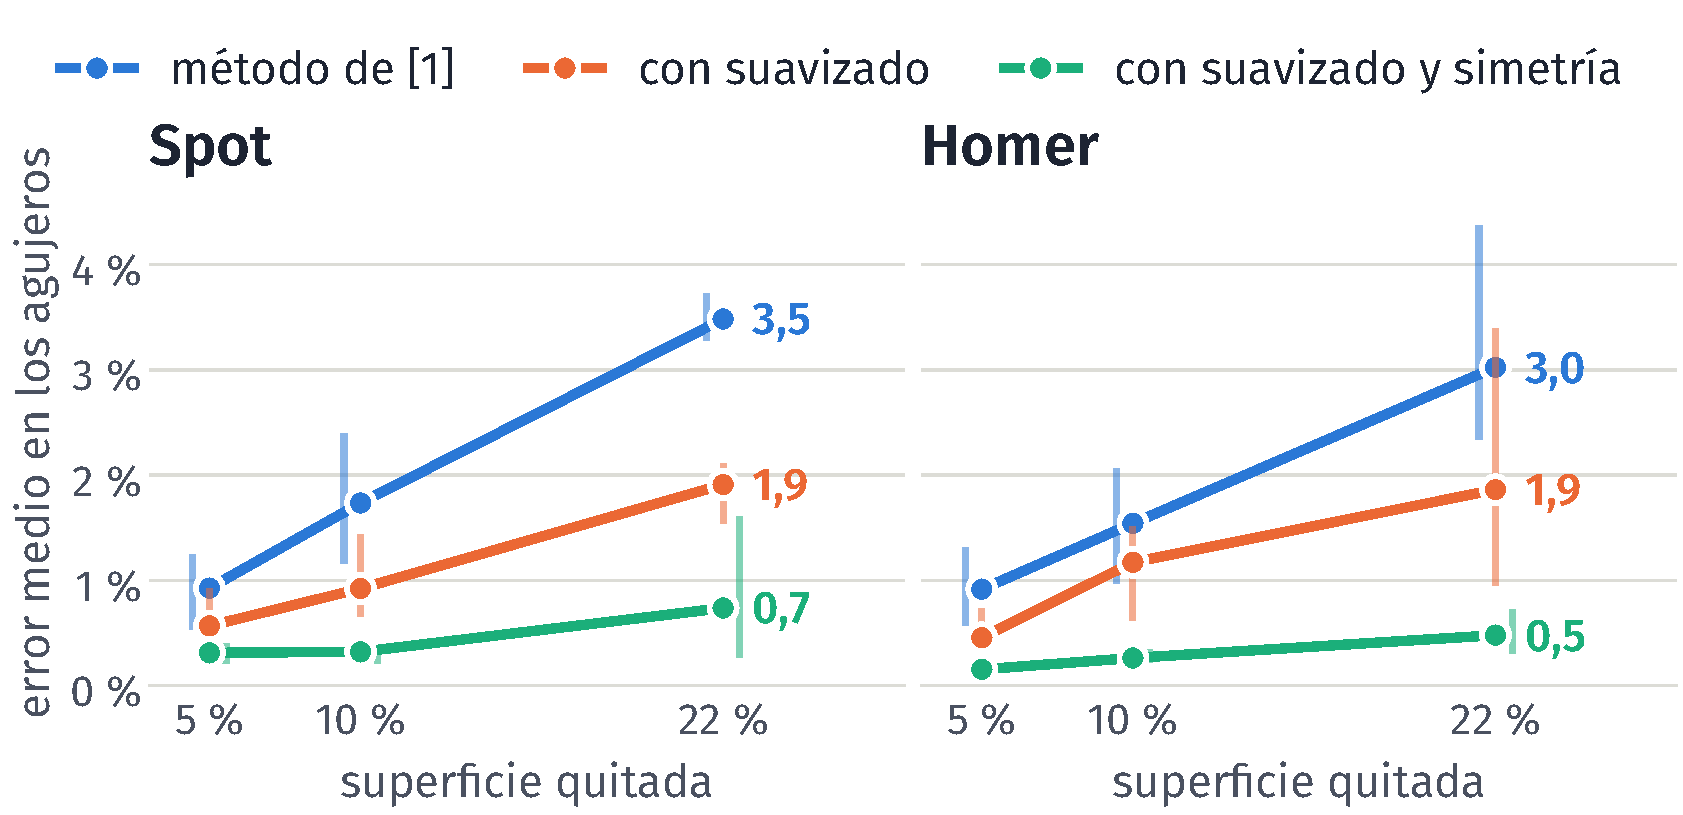
\includegraphics[width=285mm]{figuras/error.pdf}\par}

% ---------------------------------------------------------------- 4, 5 y 6
\draw[linea, line width=0.8mm] ($(current page.north west) + (25mm, -835mm)$) -- ++(650mm, 0);
\bloque{25}{845}{196}{%
  \seccion{4}{Limitaciones}
  \chico
  \punto{La simetría necesita un modelo simétrico con el otro lado sano. Si falta a ambos lados
    del plano, como la cara de Homer al 22\,\%, no hay de dónde copiar.}
  \punto{Sin simetría, el suavizado completa la forma general pero no los detalles chicos.}
  \punto{Una pieza que un agujero separa del resto sigue separada, porque el corte no controla
    la topología.}}
\bloque{243}{845}{206}{%
  \seccion{5}{Conclusiones}
  \chico
  \punto{El método de [1] decide bien qué está adentro, pero no da forma a lo que falta. Un
    suavizado local de las tapas, que no mueve la entrada, reduce el error un 43\,\%.}
  \punto{La simetría repone detalles que un suavizado no puede inventar, como la cara y la
    mano de Homer.}
  \punto{Como trabajo futuro quedan las simetrías parciales, por partes del modelo, y un corte
    de grafo que controle la topología.}}
\bloque{471}{845}{204}{%
  \seccion{6}{Referencias}
  \diminuto
  \bib{1}A.~Jacobson, L.~Kavan, O.~Sorkine-Hornung. Robust inside-outside segmentation using
  generalized winding numbers. \emph{ACM TOG} 32(4), 2013.\par
  \bib{2}H.~Si. TetGen, a Delaunay-based quality tetrahedral mesh generator. \emph{ACM TOMS}
  41(2), 2015.\par
  \bib{3}Y.~Hu et al. Tetrahedral meshing in the wild. \emph{ACM TOG} 37(4), 2018.\par
  \bib{4}M.~Botsch, L.~Kobbelt. An intuitive framework for real-time freeform modeling.
  \emph{ACM TOG} 23(3), 2004.\par
  \bib{5}X.~Li et al. Symmetry and template guided completion of damaged skulls.
  \emph{Computers \& Graphics} 35(4), 2011.\par\vspace{2mm}
  \begin{minipage}[b]{172mm}\espacios\raggedright
    Modelos: Spot (K.~Crane) y Homer (common-3d-test-models). Imágenes y mediciones
    propias.
  \end{minipage}\hfill
  \qrcode[height=27mm]{https://github.com/Lucas-Allara/MisEjercicios/tree/main/tpf}\par}

\end{tikzpicture}
\end{document}
